% !TEX program = xelatex
% !TEX root = 05_diagramme.tex
% !TEX encoding = UTF-8 Unicode
% !TEX spellcheck = de_DE
% 
% © 2016 Moritz Brinkmann, CC-by-sa
% © 2018-2022 Maximilian Jalea, CC-by-sa
% http://latexkurs.github.io

Für die Darstellung der Umfragedaten eignet sich zum Beispiel ein Säulendiagramm (|ybar|). Für die $x$-Achse würde ich die Antwort-Werte (furchtbar, meh, …) wählen. Da es sich dabei nicht um Zahlen handelt muss mit symbolischen Koordinaten gearbeitet werden. Legendeneinträge können mit \texttt{\textbackslash addlegendentry} hinzugefügt werden.


\begin{LTXexample}[pos=b,rframe={}, preset=\centering]
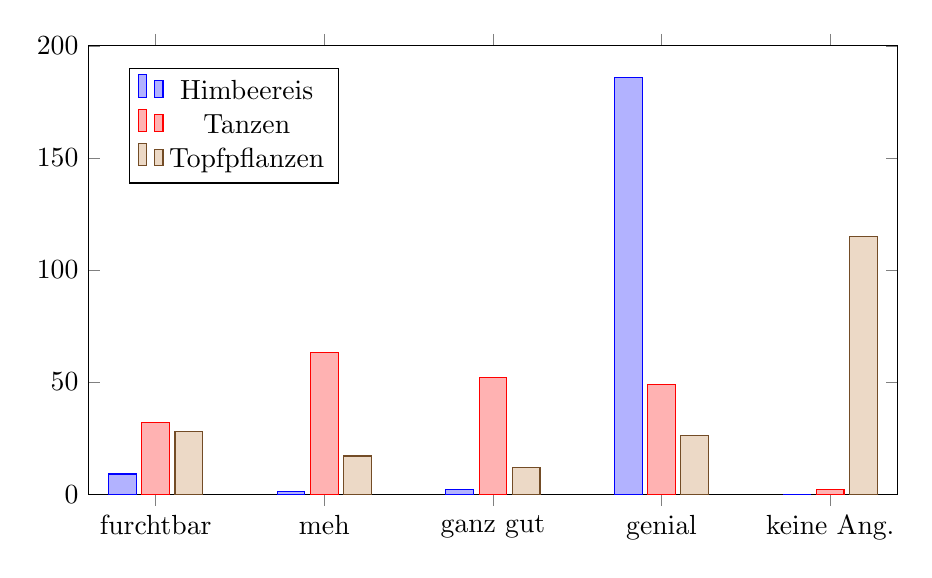
\begin{tikzpicture}
  \begin{axis}[
    ybar,
    ymin=0,
    ymax = 200,
    x post scale = 1.5,
    enlarge x limits=0.1,
    symbolic x coords={furchtbar,meh,ganz gut,genial,keine Ang.},
    xtick={furchtbar,meh,ganz gut,genial,keine Ang.},
    legend style={
      at={(0.05,0.95)},
      anchor=north west
    },
  ]
    \addplot coordinates  {(furchtbar,9) (meh,1) (ganz gut,2) (genial,186) (keine Ang.,0)};
    \addlegendentry{Himbeereis}
    
    \addplot coordinates {(furchtbar,32) (meh,63) (ganz gut,52) (genial,49) (keine Ang.,2)};
    \addlegendentry{Tanzen}
    
    \addplot coordinates {(furchtbar,28) (meh,17) (ganz gut,12) (genial,26) (keine Ang.,115)};
    \addlegendentry{Topfpflanzen}
    
  \end{axis}
\end{tikzpicture}
\end{LTXexample}
